\documentclass[
    paper=a4, 
    lang=en, 
    font=kpfonts,
    ptsize=12pt,
    titles=bf,
    hanging-titles=true,
    final
]
{skrapport} 
\colortheme{skdoc}

% meta info
\title{
    {\huge Information Theoretic Error Bounds on NISQ Learning Systems} \\
    {\large B.Tech Project I}
    }
\author[sgambhir@iitb.ac.in]{Sankalp Gambhir}
\date{\today}

% setup packages, macros, notes
\newcounter{notes}
\setcounter{notes}{1}
% general formatting and stuff
\usepackage{graphicx}
\usepackage{xcolor}
\usepackage{ragged2e}
\usepackage{ifthen}
\usepackage{lineno}
\usepackage{booktabs}
\usepackage{subcaption}

% subject specific
\usepackage{amsmath, amssymb, amsthm}
\usepackage{physics, physconst, physunits}
\newtheorem{axiom}{Axiom}

% drawing
\usepackage{pstricks}
\usepackage{tikz, tkz-orm, pgfplots}
\usetikzlibrary{arrows,shapes,backgrounds,decorations.markings}
\usetikzlibrary{matrix,positioning,decorations.pathreplacing,calc,tikzmark}
\pgfplotsset{width=7.5cm,compat=1.16}
\usepgfplotslibrary{fillbetween}

% links and citations
\usepackage{hyperref, bookmark}
\hypersetup{hidelinks} % hide boxes around links ew
\usepackage{csquotes}
\usepackage[
    style=numeric,
    sorting=none
]{biblatex}
\addbibresource{biblio.bib}

% notes
\newcommand{\notes}[1]{}

\ifthenelse{\value{notes} > 0}{
    \renewcommand{\notes}[1]{{\textcolor{red}{[Note: #1]}}}
}{}

% actual macros
\newcommand{\reals}{\ensuremath{\mathbb{R}}}
\newcommand{\naturals}{\ensuremath{\mathbb{N}}}
\newcommand{\complex}{\ensuremath{\mathbb{C}}}
\newcommand{\featurespace}{X}
\newcommand{\labelset}{L}


\begin{document}

    \begin{titlepage}
        \maketitle
        \begin{abstract}
            \lipsum[1]
        \end{abstract}        
    \end{titlepage}

    \tableofcontents \pagebreak

    \section{Introduction}
        \label{sec:intro}
        % intro.tex

% intro to problems of learning and classification
There has been long standing interest in learning from data and extrapolating
experimental data to make useful predictions using computers about as long as
computers have existed. In the last few decades, with computing power
skyrocketing exponentially coupled with leaping advances in theory of learning
systems and statistical inference, these problems became tractable and
eventually came into use ubiquitously. With applications ranging from facial
detection systems for surveillence to identifying cosmic objects for cosmology,
they have found widespread adoption in industry and academia. With their advent,
however, has come an ever rising need for computing power. This has found data
centers of unprecendented scales consuming enormous amounts of power to provide
the instant predictions we've come to rely on.

% intro to how quantum may solve it
With snowballing energy and space requirements of classical computers in the
form of GPU clusters and ASICs, there has been a spark of interest in offloading
this computation onto quantum computers, which, till recently, have largely
remained a rare species spotted only in labs surrounded by helium-cooled
superconductors and white-coated predators. Current scales of available quantum
computers, however, still lack the power required to fully tackle these
challenges while maintaining reliable error-levels or adding their own error
checking and correction. This has motivated using quantum computers to run
bottnecked computational subroutines with classical control systems. These
systems generally lack error correction, and thus earn themselves the title of
`noisy'. These form the basis of computation considered in this thesis, Noisy
Intermediate-Scale Quantum (NISQ) computers.

Connecting a quantum computer to a classical puppeteer is not expected to come
without its own issues either. It constrains the architecture and is itself
bottlenecked on both ends, first by the parameter transfer and configuration
from the classical to the quantum, then finally by the detectors on the quantum
side to the classical. In this thesis, we focus on the former, discussing the
limits of computation and computational precision achievable with this hybrid
architecture.

% report structure
\subsection{Structure}
In \autoref{sec:prelim}, definitions and relevant results in classical
computing, physics, and quantum information are presented. \notes{Extend this.}

\subsection{Outline of New Results}
\notes{Add summary of results at the end.}

    
    \section{Preliminaries}
        \label{sec:prelim}
        % prelim.tex

% classical prelims
\subsection{Classical Computing}
% learning
\subsubsection{Learning Problem}
Learning \cite{cristianini2000introduction} can be broadly defined as attempting
to learn the input-output pattern given sample data. For this thesis, we
consider three major categories of learning problems:

\begin{itemize}
    \item Binary Classification --- input points in a chosen domain, and a
    binary output label for each point.
    \item Multi-Label Classification --- input points in a chosen domain, and
    one of \(n\) labels as output for each point.
    \item Regression --- input points in a chosen domain with real-valued output.
\end{itemize}

% classification problem
\subsubsection{Classification Problem}
We take as input elements \(\{x_i\}\), generally called \emph{feature vectors},
in a chosen domain \(\featurespace\) called the \emph{feature space} and output
an element from a finite set \(\labelset = {l_i}\) of labels. \notes{Add a nice picture}

The problem is called binary classification if \(\absolutevalue{\labelset} =
2\).

Formally, we attempt to learn a function \(f: \featurespace \to \labelset\)
given a set of inputs in the domain, and possibly paired output labels.

The problem proceeds in two manners given the form of inputs: if provided
input-output pairs, the problem is called a \emph{supervised learning problem},
while attempting to learn a set of labels given just (clustered) inputs is
called \emph{unsupervised} learning. We focus on supervised classification here.

The set of input-output pairs provided is called the \emph{training data}.

Given the difficulty of working with discretized domains, the input domain is
generally converted to be a subset of a Euclidean space, using a suitable
\emph{embedding function}.

% embedding
\subsubsection{Embedding}
An embedding of \(X\) in \(Y\) is a function \(f:X \to Y\) that is injective and
structure-preserving. The exact restrictions on the map to be
structure-preserving depend on the structures of the domain and the codomain
\cite{sankappanavar1981course}. It is denoted here as \(f:X\hookrightarrow Y\).

For example, a topological embedding, i.e., the embedding of a topological
space, will be restricted to preserve its associated structure of open sets. A
field embedding, similarly, will be restricted to preserve the field operations
\(+\) and \(\times\).

For a given arbitrary feature space \(\featurespace\), it is generally embedded
into \(\reals^n\) for some \(n\).

% linear classification
\subsubsection{Linear Classification}
Classification generally proceeds by producing linear functions as candidate
(supplemented with a discretization function) labelling functions and fitting
them to the training data. For simplicity, we first restrict the discussion to
binary classifiers.

\begin{figure*}[h]
    \centering
    \begin{subfigure}{0.48\textwidth}
        % unsep bs
        \centering
        \begin{tikzpicture}[>=stealth']
            % Draw axes
            \draw [<->,thick] (0,5) node (yaxis) [above] {}
                  |- (5,0) node (xaxis) [right] {};
            % draw negative dots
            \fill[black] (0.5,1.5)    circle (3pt);
            \fill[black] (2.0,2.7)   circle (3pt);
            \fill[black] (1.0,3.4)   circle (3pt);
            \fill[black] (3.0,2.0)   circle (3pt);
            \fill[black] (1.5,1.0)   circle (3pt);
            \fill[black] (2.5,0.5)   circle (3pt);
            % draw positive dots
            \draw[black] (3.5,1.5)     circle (3pt);
            \draw[black] (2.5,1.7)     circle (3pt);
            \draw[black] (1.5,2.3)     circle (3pt);
            \draw[black] (0.5,3.0)     circle (3pt);
          \end{tikzpicture}
          \caption{Unseparated data}
    \end{subfigure}
    \begin{subfigure}{0.48\textwidth}
        % nice and separated
        \centering
        \begin{tikzpicture}[>=stealth']
            % Draw axes
            \draw [<->,thick] (0,5) node (yaxis) [above] {}
                  |- (5,0) node (xaxis) [right] {};
            % separator
            \draw (-0.5, 4.0) -- (4.0,0.0) [dashed];
            % draw negative dots
            \fill[black] (0.5,1.5)    circle (3pt);
            \fill[black] (1.5,1.7)    circle (3pt);
            \fill[black] (2.0,0.5)    circle (3pt);
            \fill[black] (1.0,2.3)    circle (3pt);
            \fill[black] (2.5,0.6)    circle (3pt);
            % draw positive dots
            \draw[black] (3.5,1.5)     circle (3pt);
            \draw[black] (2.5,2.0)     circle (3pt);
            \draw[black] (1.5,3.5)     circle (3pt);
            \draw[black] (1.0,4.0)     circle (3pt);
            \draw[black] (0.5,3.8)     circle (3pt);
          \end{tikzpicture}
          \caption{Strongly separated data}
    \end{subfigure}
    \caption{The magic of the (strong) separation axiom.}
\end{figure*}

Given a set of points which, due to an embedding, may be assumed to be in
\(\featurespace\subseteq\reals^n\), attempting to classify them may still be an
arduous task if the spatial regions corresponding to the labels are intertwined.
Thus, to make the problem tractable, we restrict the data to be \emph{strongly}
separated, i.e., any labelling function \(f:\featurespace \to \labelset\) that
agrees with the training data \notes{try to write separation properly}.

% probability distribution separation? TODO
% inner product space? TODO

% svm
\subsubsection{Support Vector Machine}
A support vector machine is a classifier model which constructs a hyperplane or
a set of hyperplanes in the feature space optimising classifier separation
depending on the objective \cite{cortes1995support}.

We will synonymously use the terms `Support Vector Machine' and that of its
common model `Maximal Margin Classifier', which is more appropriately what we
use here.

As the name suggests, a maximal margin classifier SVM tries not only to
construct a set of hyperplanes, but to find the set such that their margin from
the data is maximised. This builds upon the intuitive idea of a good separator
being further away from the given data points. See \autoref{fig:maxmargin}.


\begin{figure*}[h]
    \centering
    \begin{subfigure}{0.48\textwidth}
        % unsep bs
        \centering
        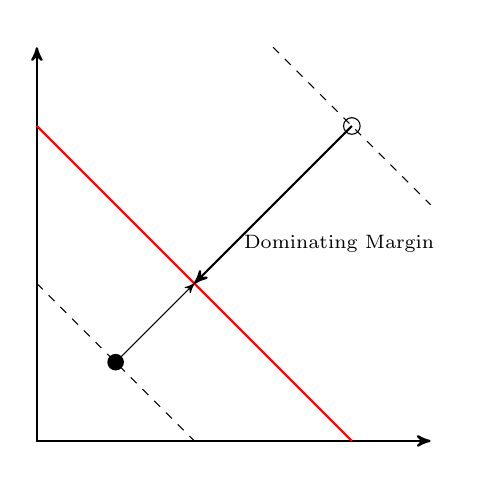
\begin{tikzpicture}[>=stealth']
            % Draw axes
            \draw [<->,thick] (0,5) node (yaxis) [above] {}
                  |- (5,0) node (xaxis) [right] {};
            % classifier
            \draw[red, thick] (0.0, 4.0) -- (4.0, 0.0);
            \draw[->, thin] (1.0, 1.0) -- (2.0, 2.0);
            \draw[->, thick] (4.0, 4.0) -- node[near end, right] {\scriptsize Dominating Margin} (2.0, 2.0);
            \draw (3.0, 5.0) -- (5.0, 3.0) [dashed];
            \draw (0.0, 2.0) -- (2.0, 0.0) [dashed];
            % draw negative dots
            \fill[black] (1,1)    circle (3pt);
            % draw positive dots
            \draw[black] (4,4)     circle (3pt);
          \end{tikzpicture}
          \caption{Unoptimized margins}
    \end{subfigure}
    \begin{subfigure}{0.48\textwidth}
        % nice and separated
        \centering
        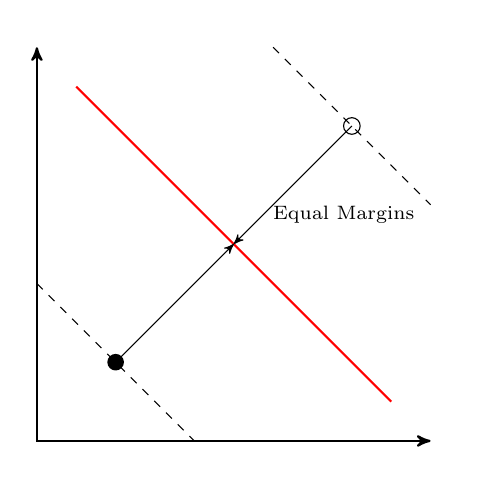
\begin{tikzpicture}[>=stealth']
            % Draw axes
            \draw [<->,thick] (0,5) node (yaxis) [above] {}
                  |- (5,0) node (xaxis) [right] {};
            % classifier
            \draw[red, thick] (0.5, 4.5) -- (4.5, 0.5);
            \draw[->] (1.0, 1.0) -- (2.5, 2.5);
            \draw[->] (4.0, 4.0) -- node[near end, right] {\scriptsize Equal Margins} (2.5, 2.5);
            \draw (3.0, 5.0) -- (5.0, 3.0) [dashed];
            \draw (0.0, 2.0) -- (2.0, 0.0) [dashed];
            % draw negative dots
            \fill[black] (1,1)    circle (3pt);
            % draw positive dots
            \draw[black] (4,4)     circle (3pt);
          \end{tikzpicture}
          \caption{Maximal margin classifier}
    \end{subfigure}
    \caption{Illustration of different margins for hyperplanes.}
    \label{fig:maxmargin}
\end{figure*}

Formally, we characterize a hyperplane in \(\reals^n\) as a pair \((\vecw, b)\),
with \(\vecw \in \reals^n\) and \(b \in \reals\), such that for all points
\(\vecx\) on the hyperplane

\begin{gather*}
    \innerprod{\vecw}{\vecx} + b = 0~.
\end{gather*}

Geometrically, \(\vecw\) is the vector normal to the hyperplane, and \(b\)
is the bias or offset from origin.

Note that by moving to \(\reals^{n+1}\), we can convert the hyperplane to one
without bias (passing through the origin)

\begin{gather*}
    \innerprod{\vecw}{\vecx} + b = 0~,\\
    \innerprod{(\vecw \oplus \begin{pmatrix}
        b
    \end{pmatrix})} {(\vecx \oplus \begin{pmatrix}
        1
    \end{pmatrix})} + 0 = 0~.
\end{gather*}

which is the hyperplane \((\vecw \oplus \begin{pmatrix}b\end{pmatrix}, 0)\) in
\(\reals^{n+1}\). So, without loss of generality, we work with hyperplanes
without bias.

Now, given the training dataset \({(\vec{x_i}, y_i)}\), with \(y_i = \pm 1\), we
can write constraints on \(\vecw\) as

\begin{gather}
    \forall i\; y_i \cdot \innerprod{\vecw}{\vec{x_i}} > 0~,
\end{gather}

that is, \(x_i\) is on the same side of the hyperplane as indicated by \(y_i\)
as the sign of the inner product corresponds to the same. 

By scaling \(\vecw\) (without changing the hyperplane), we can construct the
constraint system

\begin{gather}
    \forall i\; y_i \cdot \innerprod{\vecw}{\vec{x_i}} \geq 1~.
\end{gather}

Since we are scaling \(\vecw\), we choose an appropriate optimization target,
its norm.

Since this is a constrained optimization, we write its Lagrangian

\begin{gather}
    \mathcal{L}(\vecw, \vec{\alpha}) = \frac{1}{2} \innerprod{\vecw}{\vecw} + \sum_i \alpha_i \left[y_i \cdot \innerprod{\vecw}{\vec{x_i}}\right]~,
\end{gather}

where \(\{\alpha_i\}\) are the Lagrangian multipliers. For the optimal solution,
the Lagrangian is stationary, i.e.,

\begin{gather}
    \frac{\partial \mathcal{L}(\vecw, \vec{\alpha})}{\partial \vecw} = 0~,\nonumber\\
    \vecw - \sum_i \alpha_i y_i \vec{x_i} = 0~.
\end{gather}

Substituting this expression for \(\vecw\) in the Lagrangian itself, we get \notes{work out the substitution}

\begin{gather}
    \mathcal{L}(\vecw, \vec{\alpha}) = \frac{1}{2} \innerprod{\vecw}{\vecw} + \sum_i \alpha_i \left[y_i \cdot \innerprod{\vecw}{\vec{x_i}}\right]~,
\end{gather}

By maximising this Lagrangian with respect to the parameters \(\{\alpha_i\}\),
we obtain an optimal \(\vecw\) which is the maximum margin classifier.

With \(\vecw\) fixed at its optimal value, we get a simple computational method
to classify all new incoming points \(\vecx \in \reals^n\), given by

\begin{gather}
    \text{sgn}(\innerprod{\vecw}{\vecx})
\end{gather}

returning a label \(\pm 1\) (or anomalously zero, if you happen to pick a point
on the hyperplane, which can be remedied by making one side's boundary soft).

% how optimise
\subsubsection{Optimisation Techniques}
Gradient descent or st. \notes{expand}

% error introduction
\subsubsection{Generalisation Error}
Hello \notes{read about gen error and write here}

% qm prelims
\subsection{Quantum Regime}
\notes{add a general introduction}

% schrodinger
\subsubsection{Schr\"odinger Equation}

% hilbert space
\subsubsection{Hilbert Space}

% quantum computer
\subsubsection{Quantum Computation}

% quantum embedding
\subsubsection{State Construction and Embedding}

% measurement
\subsubsection{Measurement}

    \section{Variational Quantum Algorithms}
        \label{sec:vqa}
        % vqa.tex

% vqa structure


\begin{frame}
    \frametitle{Variational Quantum Algorithms}

    Variational Quantum Algorithms (VQA) form the idea of using a proposed
    architecture for generalised learning problems on NISQ systems
    \cite{bharti2021noisy}.

    \begin{figure}
        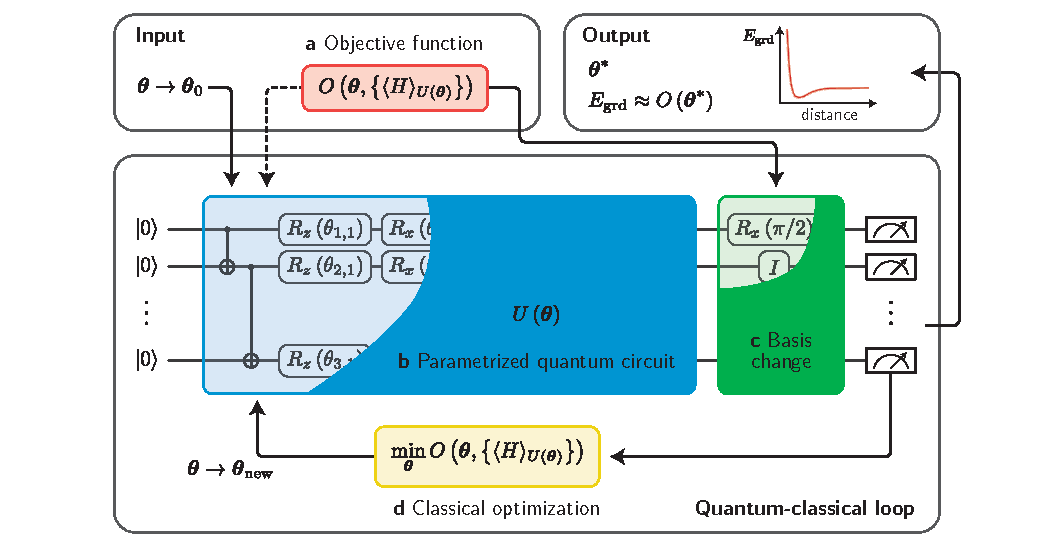
\includegraphics[width=0.8\textwidth]{figures/vqaarch.pdf}
    \end{figure}
\end{frame}

% where does this slot in?

\begin{frame}
    \frametitle{Transitioning}

    \begin{figure}
        \centering
        
        \begin{subfigure}{0.45\textwidth}
            \centering
            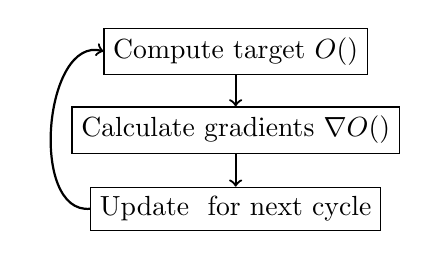
\begin{tikzpicture}[every node/.style=draw,rectangle] 
                \node (opt) [] {Compute target \(O(\vecx)\)};
                \node (grad)[below of=opt] {Calculate gradients \(\nabla O(\vecx)\)};
                \node (upd) [below of=grad] {Update \(\vecx\) for next cycle};

                \draw[->, thick] (opt) to (grad);
                \draw[->, thick] (grad) to (upd);
                \draw[->, thick, bend left=100] (upd.west) to (opt.west);
            \end{tikzpicture}
        \end{subfigure}
        %
        \pause
        \begin{subfigure}{0.45\textwidth}
            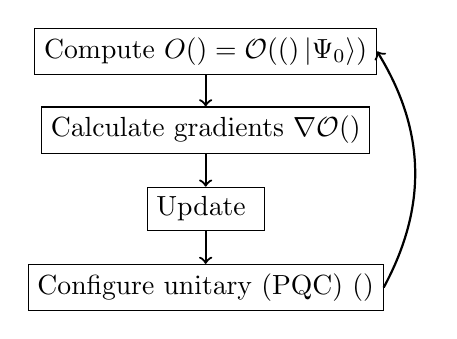
\begin{tikzpicture}[every node/.style=draw,rectangle] 
                \node (opt) [] {Compute \(O(\parameters) = \mathcal{O}(\pqc(\parameters)\ket*{\Psi_0})\)};
                \node (grad)[below of=opt] {Calculate gradients \(\nabla \mathcal{O}(\parameters)\)};
                \node (uni)[below of=grad] {Update \(\parameters\)};
                \node (upd) [below of=uni] {Configure unitary (PQC) \(\pqc(\parameters)\)};
    
                \draw[->, thick] (opt) to (grad);
                \draw[->, thick] (grad) to (uni);
                \draw[->, thick] (uni) to (upd);
                \draw[->, thick, bend right] (upd.east) to (opt.east);
            \end{tikzpicture}
        \end{subfigure}
    \end{figure}

    \begin{center}
        \(\parameters \in \reals^M, \vecx \in \reals^N, M \sim \lceil{\log_2 N}\rceil\)
    \end{center}

\end{frame}

% detailed look at PQCs
% dla
\begin{frame}
    \frametitle{Parametrized Quantum Circuits (PQCs)}

    The actual unitary computation happens in an L-layered structure with the
    mathematical form

    \begin{gather}
        \pqc(\parameters) = \prod\limits_{l = 1}^{L} U_l(\parameters_l), \quad
        \pqc_l(\parameters) = \prod\limits_{k = 1}^{K} e^{-\iota \theta_{lk} H_k}~.
        \label{eq:pqc}
    \end{gather}

    for a set of generators \(\{H_k\}\) with \(\parameters = (\parameters_1,
    \parameters_2, \ldots, \parameters_k)\).

    \pause
    Formally, the generators create a Dynamical Lie Algebra, which determines
    the set of reachable unitaries. The choice of generators can strongly affect
    the optimization process \cite{larocca2021diagnosing}. See the report for a
    detailed study.

\end{frame}

% qlt
\begin{frame}
    \frametitle{Quantum Landscape Theory}

    Spaces and maps involved in VQA calculation \cite{larocca2021theory}:

    \begin{figure}
        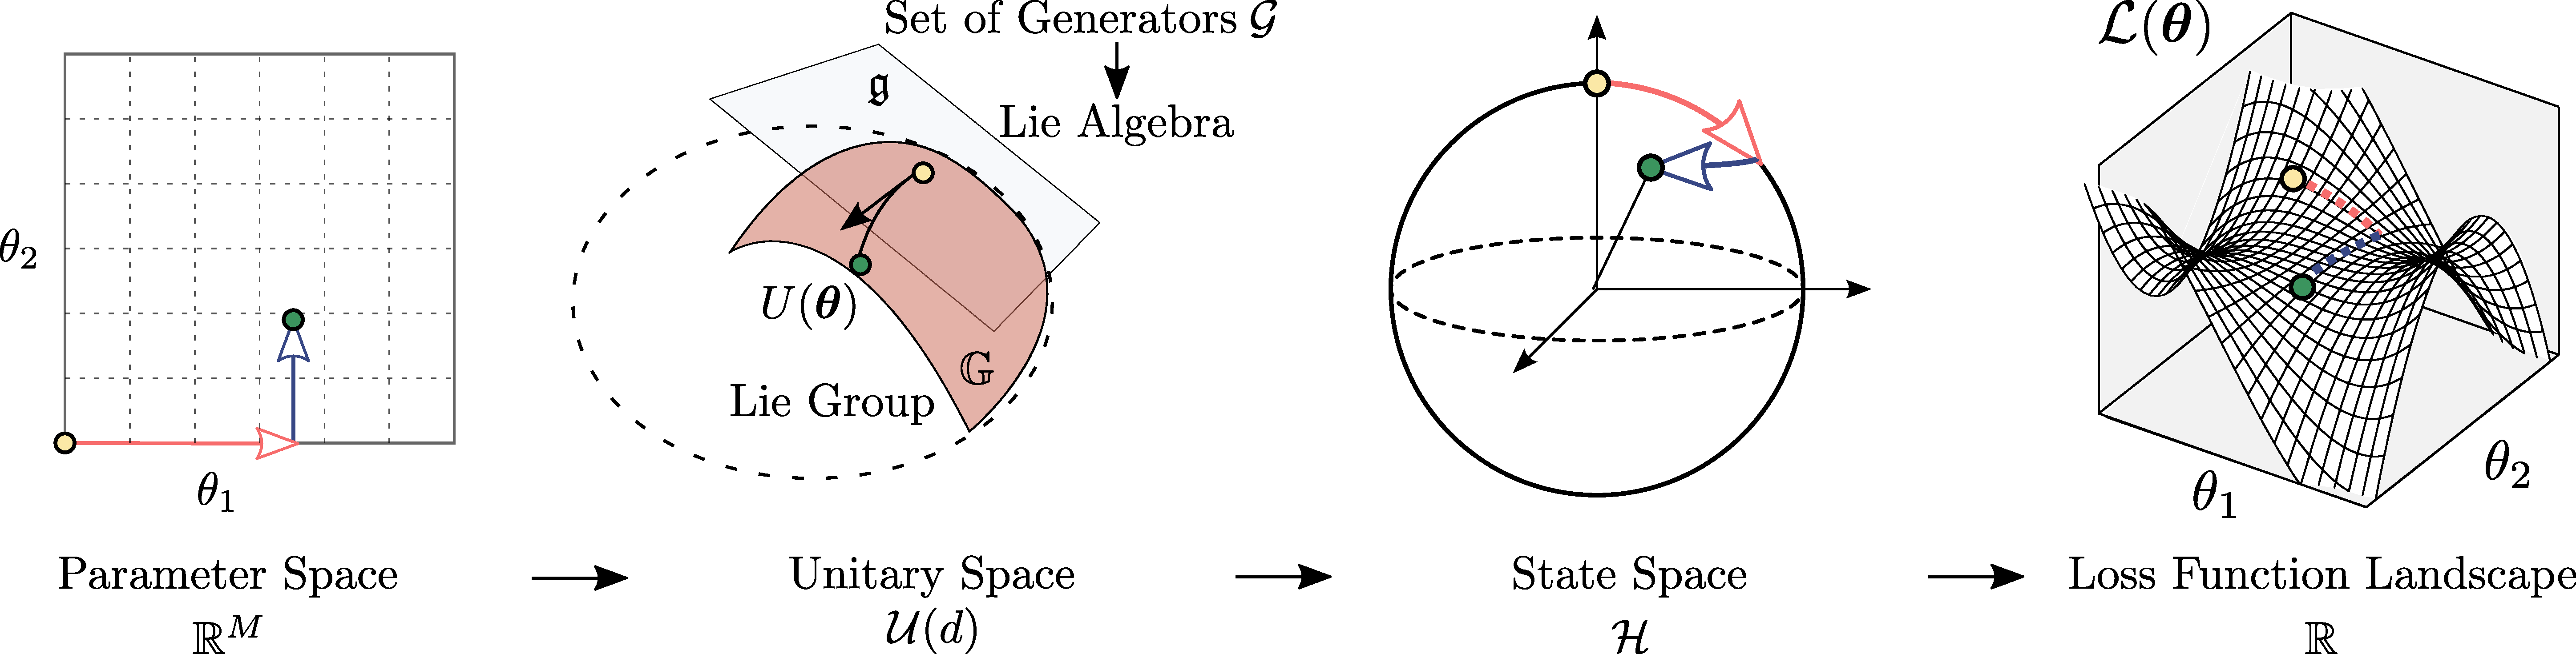
\includegraphics[width=0.8\textwidth]{figures/mapsurjective.pdf}
    \end{figure}

    This structure forms the playground for our analysis. The study of these
    spaces forms an important part of establishing relative bounds at stages of
    the calculation (which are the spaces). We discuss the particular case of
    \(\mathcal{U}(d) \to \hilbertspace\) here. See the report for details on the
    other maps.

\end{frame}

    
    \section{Information Theoretic Limits}
        \label{sec:infolimits}
        % infolimits.tex

Having proposed a structure to solve learning problems with a NISQ system, we
are ill-fated to then deal with the myriad of issues that arise with daring to
use it. Barring issues specific to the quantum states, low coherence times,
inaccurate measurements, et cetera, our structure itself
imposes some bottlenecks on what we can achieve with it. In particular, the act
of converting and transferring data between the representations used by the
quantum and classical halves induces the issue of information transfer and
limits upon it. 

The idea of information theoretic bounds goes back to the father of information
theory, Claude Shannon himself \cite{shannon1948mathematical}. Work from
Nyquist, Hartley, and Shannon \cite{hartley1928transmission} built up the
structure of information theory to quantify the maximum `amount of data' that
could be transferred through a noisy communications channel and the changes to
said effective `amount' on the implementation of error correcting codes over the
channel.

The analysis for the hybrid computing case has partially been performed in a
general setting \cite{lloyd2014information}. The authors suggest in the paper an
extension to construction of unitaries, but do not explore it further. To the
best of our knowledge, this has not been discussed in other literature since.
Here, we continue the discussion for the specific case of VQAs with the goal to
parametrize the discussion with circuit characteristics (depth, width, DLA) and
discuss the bounds on VQA computation from the optimal control theorems
presented in the paper.

\subsection{Summary of Bounds on Quantum Optimal Control}
A quantum system (target of control) can be presented as a dynamical equation

\begin{equation}
    \dot{\rho} = \mathcal{L}(\rho, \controlpulse(t))~,
\end{equation}

where \(\rho\) is the density matrix representing the current state of the
system, \(\dot{\rho}\) its time evolution, \(\controlpulse\) the externally
applied control pulse, and \(\mathcal{L}\), here, the resulting Liouvillian
superoperator \cite[see][section IV]{manzano2020lindblad}. The same notation is
used for the loss function earlier, and is kept here only to be consistent with
the source. The two will not be used together in this thesis.

The dynamics are subject to the boundary condition \(\rho(t=0) = \rho_0\), and
the unitary part of \(\mathcal{L}\) must be generated by a Hamiltonian

\begin{equation}
    \hamiltonian = \hamiltonian_D + \controlpulse(t) \hamiltonian_C~,
\end{equation}

where \(\hamiltonian_D\) and \(\hamiltonian_C\) are the drift and control
Hamiltonians respectively. The dynamics can be generalized to have several
control Hamiltonians and corresponding pulses, but the extension is
straightforward and skipped here for simplicity.

Now, for choices of the control pulse \(\controlpulse\), define the set of
reachable states as the set \(\reachable\), a manifold with dimension
\(\dimD_\reachable\), which is a subset of the space of density matrices of
dimension \(\dimD_\rho\), with of course \(\dimD_\reachable \leq \dimD_\rho\).
Thus, given a goal state \(\bar{\rho}\), and an initial state \(\rho_0\) the
problem is to find a (not necessarily unique) optimal control pulse
\(\bar{\controlpulse}\) such that it drives the initial state to a final state
within an \(\epsilon\)-ball around the goal state. This can be written as a
functional minimization

\begin{equation}
    \bar{\rho}(t) = \text{arg min}_{\controlpulse(t)} 
    \mathcal{F}(\rho_0, \bar{\rho}, \controlpulse(t), [\lambda_i])~,
\end{equation}

where the functional \(\mathcal{F}\) quantifying the distance between states may
also include constraints introduced via the Lagrangian multipliers
\(\{\lambda_i\}\).

To the end of this optimization, suppose one adjusts the control pulse with a
classical channel. In the ideal noiseless case, Hartley's Law bounds the
information transfer as

\begin{equation}
    b_\gamma = T\Delta\Omega\kappa_s~,
\end{equation}

where \(T\) is the pulse duration, \(\Delta\Omega\) the bandwidth, and
\(\kappa_s\) is the bit depth of the pulse. With the control pulse \(\gamma\)'s
extreme levels as \(\gamma_{max}\) and \(\gamma_{min}\), define \(\Delta\gamma =
\gamma_{max} - \gamma{min}\). Finally, set the minimum variation to be
\(\delta\gamma\). Then,

\begin{equation}
    \kappa_s = \text{log}(1+\frac{\Delta\gamma}{\delta\gamma})~.
\end{equation}

These parameters can be used to give an error bound on the achievable state
\(\norm{\rho - \bar{\rho}} > \epsilon\), with

\begin{equation}
    \epsilon \geq 2^{-\frac{T\Delta\Omega\kappa_s}{\dimD_\polyreachable}}~.
\end{equation}

For a detailed build up to the results, see \cite{lloyd2014information}.

\subsection{Bounds on PQC Optimization}

Similar to the Optimal Control scenario, the VQA architecture also presents the
same infrastructural bounds. It stands to reason that a similar result should
extend to generation of unitaries using a PQC. This is suggested in
\cite{lloyd2014information}, but not explored further. We seek to establish
lower bounds on the information theoretic error on learning the unitaries in
terms of the circuit parameters --- circuit width, depth, and choice of
generators (ansatz).

The bound requires establishing a distance and measure in the DLA to bound the
number of \(\epsilon\)-balls required to cover the space. A candidate for this
study is the idea of a Haar measure \cite{van1995haar}. Extending this result to
usable bounds for the outputs requires further study of the maps discussed in
\autoref{subsec:quantlandscape}. A preliminary result over the state space is
discussed in \autoref{sec:qsvm}.

An alternate possible computation could use an error bound in real space
\(\reals^M\) and use the map in \autoref{subsec:quantlandscape} to the unitary
group to find an extended bound. This is much simpler compared to the ab initio
calculation but does not necessarily give an exact bound.


    \section{Applications - Quantum Support Vector Machine}
        \label{sec:qsvm}
        % qsvm.tex

Given training data embedded as n-qubit quantum states \(\{\ket*{x_i}\}\) with
corresponding labels \({y_i = \pm 1}\), a QSVM implemented as a VQA attempts to learn a
unitary \(\pqc(\parameters)\) such that

\begin{equation}
    \text{sgn }{\bra*{0}^{\otimes n}\pqc(\parameters)^*\ket*{x_i}} = y_i \forall i~.
\end{equation}

Setting \(\ket*{w} = \pqc(\parameters)\ket*{0}^{\otimes n}\) recovers the
familiar classical SVM from \autoref{eq:svmclassifier}.

An \(\epsilon\) error in the unitary correspondingly generates an error in
\(\ket*{w}\) and generates a conical section (more generally, a hypersector of
an n-hypersphere) as seen in \autoref{fig:qsvmerrorcone}.

\begin{figure}[!ht]
    % error cones
    \centering
    \begin{tikzpicture}[>=stealth']
        % Draw axes
        \draw [<->,thick] (0,5) node (yaxis) [above] {}
              |- (5,0) node (xaxis) [right] {};
        \draw [<->,thick] (0,-5) node (negyaxis) [above] {}
              |- (-5,0) node (negxaxis) [right] {};
        % classifier
        \draw[red, thick] (-4, -4) -- (4, 4);
        \draw[red, thick,->] (0, 0) -- node[very near end, right] {\(~\ket*{w}\)} (+1, -1);
        % error bars
        \draw (-3.5, -4.5) -- (3.5, 4.5) [dashed];
        \draw[->] (0, 0) -- (1.2, -0.8)[dashed];
        \draw (-4.5, -3.5) -- (4.5, 3.5) [dashed];
        \draw[->] (0, 0) -- node[very near end, below] {\(\ket*{w_\epsilon}\)} (0.8, -1.2)[dashed];
      \end{tikzpicture}
      \caption{Intuitive representation of error in the hyperplane normal vector.}
      \label{fig:qsvmerrorcone}
\end{figure}

Picking a point randomly in the space outside the training data and attempting
to classify it, we find an error probability proportional to the volume of the
hypersector generated by the error in \(\ket*{w}\). We have using volume
formulae from \cite{li2011concise}

\begin{align}
        p_{\text{error}} &= \lim_{r\to \infty}\frac{2\cdot V_{\text{sector}}(r)}{V_{\text{sphere}}(r)} \nonumber\\
            &= \lim_{r\to \infty}\frac{2\cdot V_{\text{sphere}}(r)\cdot 0.5\cdot I_{\text{sin}^2\phi}(\frac{n-1}{2}, \frac{1}{2})}{V_{\text{sphere}}(r)} \nonumber\\
            &= I_{\text{sin}^2\phi}(\frac{n-1}{2}, \frac{1}{2})~,
\end{align}

where \(I\) is the incomplete Beta function, 

\begin{equation}
    I_x(a, b) = \frac{B(x; a, b)}{B(a, b)} = \frac{\int_0^x t^{a-1} (1-t)^{b-1} \dd t}{\int_0^1 t^{a-1} (1-t)^{b-1} \dd t}~,
\end{equation}

and \(\phi\) is the angular distortion, and it is seen from \(\ket*{w} =
\pqc(\parameters)\ket*{0}\) that \(\text{sin} \phi \sim \epsilon\). Finally, we
have,

\begin{equation}
    p_{\text{error}} \sim I_{\epsilon^2}(\frac{n-1}{2}, \frac{1}{2})~.
\end{equation}

For a fixed \(\epsilon\), this error probability falls off quite quickly with
\(n\). See \autoref{fig:perrorplot} for plots of the probability with varying
\(n\) at different values of \(\epsilon\). The form of the function suggests
that while there is a fundamental limit to learning the unitaries, it may not
always be a hindrance to be wary of, provided the system is of sufficiently
high dimension.

\begin{figure}
    \centering
    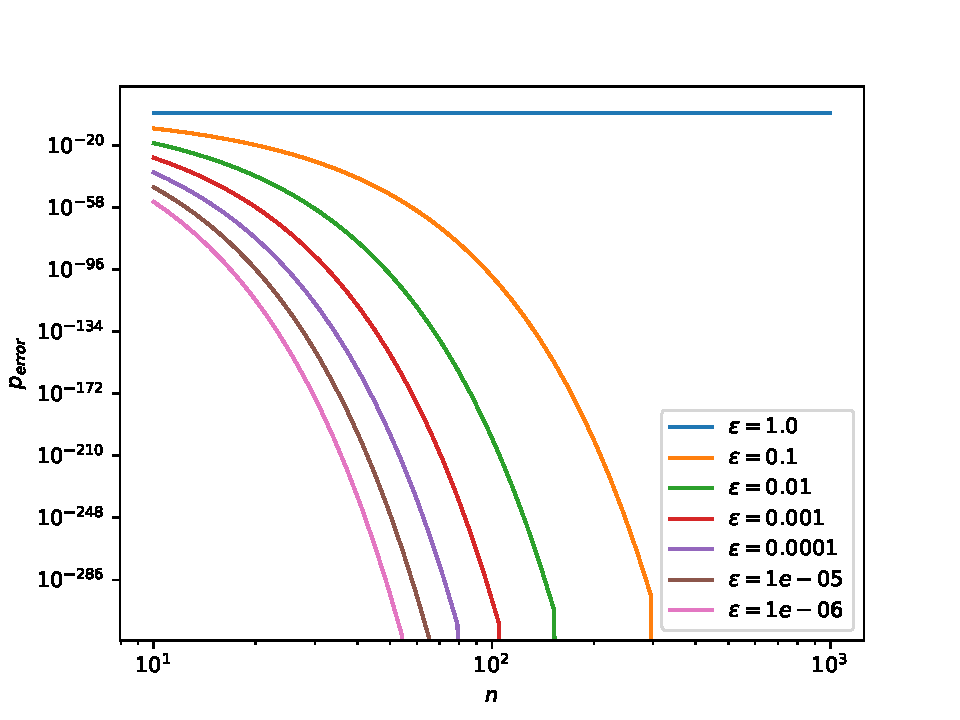
\includegraphics[width=0.8\textwidth]{figures/perrorplot.pdf}
    \caption{\(p_{\text{error}}\) with change in \(n\) at several values of \(\epsilon\).}
    \label{fig:perrorplot}
\end{figure}

However, it is to be noted that this analysis uses a fixed value of the unitary
distortion, \(\epsilon\). In a real system, this is certainly not expected to be
independent of the circuit width (number of qubits, dimension of state space).
Preliminary calculations as described in \autoref{sec:infolimits} suggest that
\(\epsilon\) is a function of the circuit area, i.e., the circuit width and
depth product. This is related to the quantity \(M\) described in
\autoref{subsubsec:pqc}. So, an increase in width correspondingly leads to a
\emph{decrease} in depth of the circuit to maintain the same error bounds for
the unitary output.

The depth of the circuit has been heavily correlated to the barren plateau
problem \cite{larocca2021theory}. Increasing the depth of the circuit has been
identified to remove spurious minimas from the problem and overparametrization
beyond a certain depth (characterized by the QFIM) leads to deepening of present
minimas, with a tradeoff towards barren plateaus \cite{larocca2021diagnosing}.
This new result presents a second tradeoff. If we keep the error constant, and
thus by the hypothesis, the area, the reduction in error by increase in width
(upto a certain level, see \autoref{fig:perrorplot}) would require a decrease in
depth, leading to spurious minimas. This tradeoff is a subject of our current
study.

\begin{figure}[ht]
    \centering
    %
    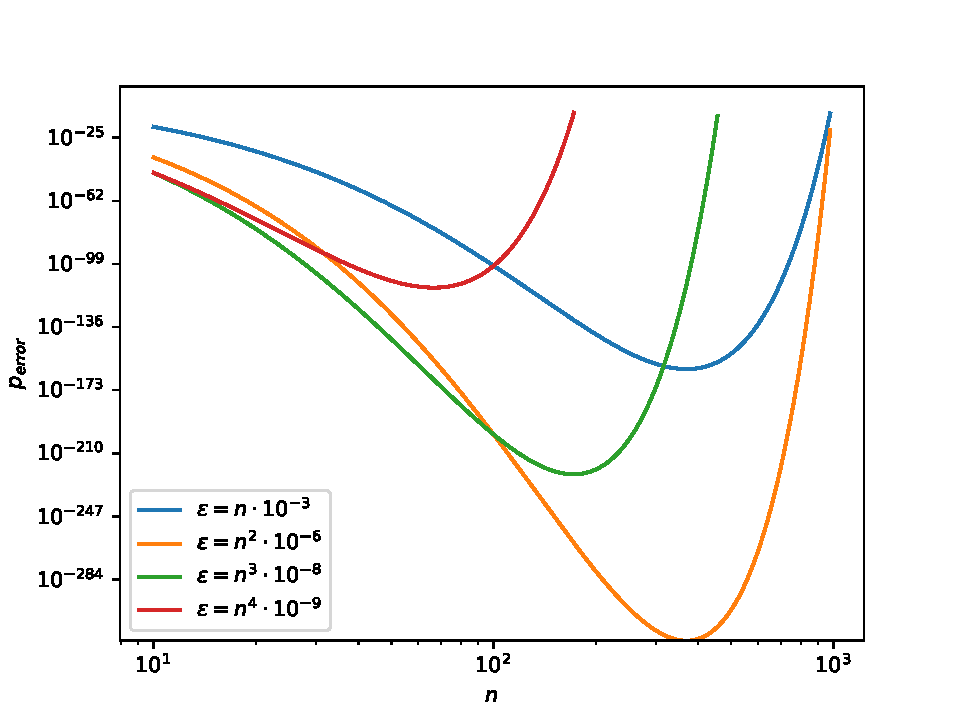
\includegraphics[width=0.8\textwidth]{figures/perrorscaled.pdf}
    \caption{\(p_{\text{error}}\) scaling assuming \(\epsilon\) changes with \(n\).}
    \label{fig:perrorscaled}
\end{figure}

For illustration, values of the error probability are plotted in
\autoref{fig:perrorscaled} with different scaling functions chosen for
\(\epsilon\) dependent on n, assuming a fixed circuit depth. Note that this
calculation suggests the existence of a width (number of qubits) for a given
depth and circuit configuration where generealisation error is minimized.


    \section{Conclusion and Future Work}
        \label{sec:future}
        % future.tex

In this report we reviewed Variational Quantum Algorithms and classification
theory, finally establishing error bounds on the output of a Quantum Support
Vector Machine supported by a VQA backend. We are continuing work on studying
the landscape generated by the Dynamical Lie Algebra and consequently to pull
back the error bounds to the unitary group to propose bounds generalized from
the QSVM to the Parametrized Quantum Circuit. Next steps involve literature
review and study of compact group measures and the information content of those
descriptions. With a more formalized mathematical description of the landscaping
maps in terms of measure theory, the problem of reporting error bounds at each
step of the computation is expected to be tractable.

    \phantomsection
    \addcontentsline{toc}{section}{References}
    \printbibliography
\end{document}